\part{Práctica 4}

\section{Ejercicio 1}
\begin{center}
    \parbox{12cm}{\justify\textit{Uso extendido de GNU/Linux en escritorio y en la industria. Últimos avances.
    Lectura recomendada:
    \begin{itemize}
        \item \href{https://hipertextual.com/2018/12/snaps-instalar-software-linux}{Snaps: ¿El método más simple para instalar apps en Linux?}
    \end{itemize}
    Cuestiones:
    \begin{enumerate}
    \item Porcentaje de uso de los principales SO de escritorio.
    \item ¿Cómo crees que podría mejorarse el uso de GNU/Linux en escritorios?
    \item ¿Qué es snap y snapcraft.io? ¿para qué sirve y qué diferencias aporta al sistema tradicional de instalación de paquetes de GNU/Linux?
    \item Buscar cómo se instala snap en mi distribución en la documentación de snap.
    \item Instalar y probar snap
    \item ¿Crees que mejora en el sentido de facilitar el uso de GNU/Linux?
    \end{enumerate}}}
\end{center}

\subsection{Pregunta 1}
Estos gráficos muestran los datos de abril de 2020 sobre el porcentaje de uso de los principales SO de escritorio en todo el mundo \cite{statcounter:os_share_worldwide} y en España \cite{statcounter:os_share_spain}.
\begin{figure}[H]
    \centering
    \begin{tikzpicture}    
        \pie [cloud, scale font, radius=2, text=legend]
        {76.5/Windows, 18.99/OS X, 1.61/Linux, 1.12/Chrome OS, 1.75/Otros}
    \end{tikzpicture}
    \caption{Uso de los principales SO de escritorio en abril de 2020 en el mundo.}\label{fig:uso-so-mundial}
\end{figure}
\begin{figure}[H]
    \centering
    \begin{tikzpicture}    
        \pie [cloud, scale font, radius=2, text=legend]
        {76.1/Windows, 20.62/OS X, 1.71/Linux, 0.46/Chrome OS, 1.11/Otros}
    \end{tikzpicture}
    \caption{Uso de los principales SO de escritorio en abril de 2020 en España.}\label{fig:uso-so-españa}
\end{figure}

\subsection{Pregunta 2}
Sin duda, el principal factor que mejoraría el porcentaje de uso de GNU/Linux a largo plazo es la adopción por parte de las administraciones, sobre todo en el ámbito de la educación. Por otra parte, la mayoría de los ordenadores que se venden incluyen una licencia de Windows como si no hubiera opción. Si se acabase con esta práctica y en su lugar se permitiese al comprador elegir, los usuarios percibirían mejor el valor y el precio del producto que están comprando y, sin duda, muchos elegirían GNU/Linux aunque sólo fuera por el precio.

En mi opinión, la dificultad de uso no es un factor que frene la adopción de GNU/Linux para el usuario medio de hoy. Si algo detiene al usuario a la hora de decidir utilizar un sistema operativo diferente es hábito, el aferrarse a lo que conoce y rechazar el cambio.

\subsection{Pregunta 3}
<<Snap>> es un sistema de gestión de paquetes paquete de aplicación para escritorio, nube o IoT, creado y diseñado por Canonical. \href{http://snapcraft.io}{snapcraft.io} es la herramienta que utilizan los desarrolladores para empaquetar sus programas en formato snap.
La principal ventaja de snap frente a otros sistemas de gestión de paquetes es ser independiente de la distribución en la que se instala. Los propios snaps no dependen de ninguna tienda de aplicaciones y se pueden obtener de cualquier forma. El inconveniente de Snap es el mayor tamaño de sus paquetes, ya que cada uno viene con sus dependencias incluidas.

\subsection{Pregunta 4}
Según las instrucciones para la \href{https://snapcraft.io/docs/installing-snap-on-ubuntu}{instalación de snap en Ubuntu}\footnote{\label{nota1}\url{https://snapcraft.io/docs/installing-snap-on-ubuntu}}, snap se instala por defecto en Ubuntu 20.04, que es la distribución que tengo actualmente instalada.

\subsection{Pregunta 5}
Como snap se instaló automáticamente con mi Ubuntu, paso a comprobar la instalación siguiendo las instrucciones que dan en \href{https://snapcraft.io/docs/installing-snap-on-ubuntu}{snapcraft.io}\footnotemark[1]. En la figura \ref{fig:ubuntu-snap} se puede ver la ejecución del comando snap sin parámetros, la instalación del paquete \code{hello-world} y la ejecución posterior del programa instalado.

\begin{figure}[H]
    \centering
    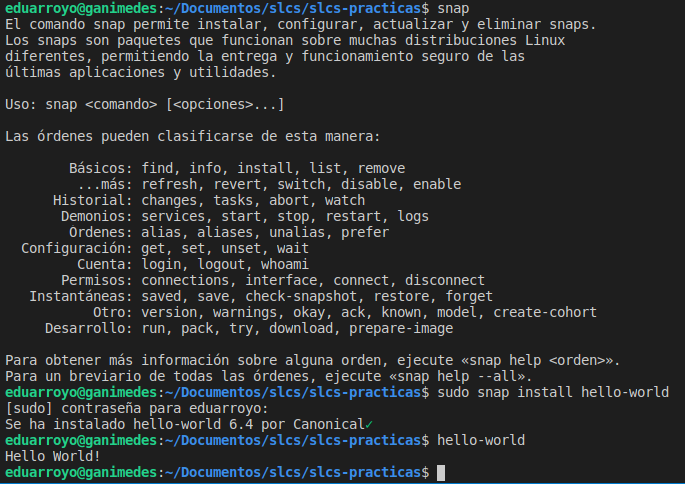
\includegraphics[scale=0.5]{comprobacion-ubuntu-snap}
    \caption{Comprobación de funcionamiento de snap}
    \label{fig:ubuntu-snap}
\end{figure}

\subsection{Pregunta 6}
Al menos en Ubuntu, la tienda de aplicaciones que conocía, junto con \code{npm}, el conocido gestor de paquetes, hacían bastante fácil la instalación de aplicaciones en GNU/Linux. Sin duda, el carácter multiplataforma de snap contribuye a una mayor homogeneización del software entre las distintas distribuciones, pero sobre todo facilita el trabajo a los desarrolladores, que sólo tienen que empaquetar sus aplicaciones en un sistema.

\section{Ejercicio 2}
\begin{center}
    \parbox{12cm}{\justify\textit{Free software and GNU/Linux publications:
    \begin{itemize}
    \item LJ. Linux Journal. \url{https://www.linuxjournal.com/}
    \item LM. Linux Magazine. \url{http://www.linux-magazine.com/}
    \item Linux Weekly News. \url{https://lwn.net/}
    \item \url{http://linux.com}
    \item nixCraft. \url{https://www.cyberciti.biz/}
    \item \href{https://slashdot.org}{slashdot} y barrapunto
    \item OMG! Ubuntu!. We follow the Ubuntu and GNOME development. \url{https://www.omgubuntu.co.uk/}
    \item Sección “Linux” en: \url{http://hipertextual.com}
    \item \url{https://ayudalinux.com/}
    \item \url{https://lamiradadelreplicante.com/}
    \end{itemize}
    Cuestiones:
    \begin{enumerate}
    \item Ordena tus preferencias de 1 a 5.
    \item ¿Has encontrado contenido GNU/Linux o de free software en otras publicaciones?¿Cuáles?
    \end{enumerate}}}
\end{center}


\section{Ejercicio 3}
\begin{center}
    \parbox{12cm}{\justify\textit{GNU/Linux en redes sociales:
    \begin{itemize}
    \item \href{https://twitter.com/Linux}{@Linux} 269mil
    \item \href{https://twitter.com/usemoslinux}{@usemoslinux} 24mil
    \item \href{https://twitter.com/MuyLinux}{@MuyLinux} 23mil
    \item \href{https://twitter.com/linuxhispano}{@linuxhispano} 7mil
    \item \href{https://twitter.com/andalinux}{@andalinux} 3mil
    \item \href{https://twitter.com/AulaSL}{@AulaSL} 634
    \end{itemize}
    Best Linux hashtags, o hashtags relacionadas con Linux que más se usan en RRSS:
    \href{https://twitter.com/hashtag/linux}{\#linux}
    \href{https://twitter.com/hashtag/programming}{\#programming}
    \href{https://twitter.com/hashtag/python}{\#python}
    \href{https://twitter.com/hashtag/coding}{\#coding}
    \href{https://twitter.com/hashtag/hacking}{\#hacking}
    \href{https://twitter.com/hashtag/technology}{\#technology}
    \href{https://twitter.com/hashtag/programmer}{\#programmer}
    \href{https://twitter.com/hashtag/technology}{\#technology}
    \href{https://twitter.com/hashtag/java}{\#java}
    \href{https://twitter.com/hashtag/hacker}{\#hacker}
    \href{https://twitter.com/hashtag/computerscience}{\#computerscience}
    \href{https://twitter.com/hashtag/code}{\#code}
    \href{https://twitter.com/hashtag/coder}{\#coder}
    \href{https://twitter.com/hashtag/javascript}{\#javascript}
    \href{https://twitter.com/hashtag/html}{\#html}
    \href{https://twitter.com/hashtag/developer}{\#developer}
    \href{https://twitter.com/hashtag/cybersecurity }{\#cybersecurity }
    \href{https://twitter.com/hashtag/webdeveloper}{\#webdeveloper}
    \href{https://twitter.com/hashtag/css}{\#css}
    \href{https://twitter.com/hashtag/computer}{\#computer}
    \href{https://twitter.com/hashtag/kalilinux}{\#kalilinux}
    \href{https://twitter.com/hashtag/software}{\#software}
    \href{https://twitter.com/hashtag/php}{\#php}
    \href{https://twitter.com/hashtag/webdevelopment}{\#webdevelopment}
    \href{https://twitter.com/hashtag/webdesign}{\#webdesign}
    \href{https://twitter.com/hashtag/programmers}{\#programmers}
    \href{https://twitter.com/hashtag/geek}{\#geek}
    \href{https://twitter.com/hashtag/softwaredeveloper}{\#softwaredeveloper}
    \href{https://twitter.com/hashtag/windows}{\#windows}
    \href{https://twitter.com/hashtag/bhfyp}{\#bhfyp}
    \\
    Cuestiones:
    \begin{enumerate}
    \item Anota las cuentas de Twitter que más te gusten de las anteriores o de otras que tú consultes en orden preferente de 1 a 5.
    \item ¿Has encontrado contenido GNU/Linux o de free software en otras RRSS? ¿Cuáles?
    \end{enumerate}
    Lectura recomendada en el portal Linux Journal sobre su 25 aniversario:
    \begin{itemize}
        \item \href{https://www.linuxjournal.com/content/25-years-later-interview-linus-torvalds}{25 Years Later: Interview with Linus Torvalds}
    \end{itemize}
    }}
\end{center}